\documentclass{extbook}[14pt]
\usepackage{multicol, enumerate, enumitem, hyperref, color, soul, setspace, parskip, fancyhdr, amssymb, amsthm, amsmath, bbm, latexsym, units, mathtools}
\everymath{\displaystyle}
\usepackage[headsep=0.5cm,headheight=0cm, left=1 in,right= 1 in,top= 1 in,bottom= 1 in]{geometry}
\usepackage{dashrule}  % Package to use the command below to create lines between items
\newcommand{\litem}[1]{\item #1

\rule{\textwidth}{0.4pt}}
\pagestyle{fancy}
\lhead{}
\chead{Answer Key for Progress Quiz 4 Version B}
\rhead{}
\lfoot{4378-7085}
\cfoot{}
\rfoot{Fall 2020}
\begin{document}
\textbf{This key should allow you to understand why you choose the option you did (beyond just getting a question right or wrong). \href{https://xronos.clas.ufl.edu/mac1105spring2020/courseDescriptionAndMisc/Exams/LearningFromResults}{More instructions on how to use this key can be found here}.}

\textbf{If you have a suggestion to make the keys better, \href{https://forms.gle/CZkbZmPbC9XALEE88}{please fill out the short survey here}.}

\textit{Note: This key is auto-generated and may contain issues and/or errors. The keys are reviewed after each exam to ensure grading is done accurately. If there are issues (like duplicate options), they are noted in the offline gradebook. The keys are a work-in-progress to give students as many resources to improve as possible.}

\rule{\textwidth}{0.4pt}

\begin{enumerate}\litem{
Determine the domain of the function below.
\[ f(x) = \frac{5}{30x^{2} +10 x -20} \]
The solution is \( \text{All Real numbers except } x = -1.000 \text{ and } x = 0.667. \), which is option B.\begin{enumerate}[label=\Alph*.]
\item \( \text{All Real numbers except } x = a, \text{ where } a \in [-1.2, 0.2] \)

All Real numbers except $x = -1.000$, which corresponds to removing only 1 value from the denominator.
\item \( \text{All Real numbers except } x = a \text{ and } x = b, \text{ where } a \in [-1.2, 0.2] \text{ and } b \in [-0.6, 1.1] \)

All Real numbers except $x = -1.000$ and $x = 0.667$, which is the correct option.
\item \( \text{All Real numbers except } x = a \text{ and } x = b, \text{ where } a \in [-25.3, -23.6] \text{ and } b \in [22.9, 24.3] \)

All Real numbers except $x = -25.000$ and $x = 24.000$, which corresponds to not factoring the denominator correctly.
\item \( \text{All Real numbers except } x = a, \text{ where } a \in [-25.3, -23.6] \)

All Real numbers except $x = -25.000$, which corresponds to removing a distractor value from the denominator.
\item \( \text{All Real numbers.} \)

This corresponds to thinking the denominator has complex roots or that rational functions have a domain of all Real numbers.
\end{enumerate}

\textbf{General Comment:} Recall that dividing by zero is not a real number. Therefore the domain is all real numbers \textbf{except} those that make the denominator 0.
}
\litem{
Determine the domain of the function below.
\[ f(x) = \frac{4}{15x^{2} -43 x + 30} \]
The solution is \( \text{All Real numbers except } x = 1.200 \text{ and } x = 1.667. \), which is option B.\begin{enumerate}[label=\Alph*.]
\item \( \text{All Real numbers.} \)

This corresponds to thinking the denominator has complex roots or that rational functions have a domain of all Real numbers.
\item \( \text{All Real numbers except } x = a \text{ and } x = b, \text{ where } a \in [0.77, 1.29] \text{ and } b \in [1.65, 1.95] \)

All Real numbers except $x = 1.200$ and $x = 1.667$, which is the correct option.
\item \( \text{All Real numbers except } x = a, \text{ where } a \in [14.66, 15.62] \)

All Real numbers except $x = 15.000$, which corresponds to removing a distractor value from the denominator.
\item \( \text{All Real numbers except } x = a, \text{ where } a \in [0.77, 1.29] \)

All Real numbers except $x = 1.200$, which corresponds to removing only 1 value from the denominator.
\item \( \text{All Real numbers except } x = a \text{ and } x = b, \text{ where } a \in [14.66, 15.62] \text{ and } b \in [29.92, 30.14] \)

All Real numbers except $x = 15.000$ and $x = 30.000$, which corresponds to not factoring the denominator correctly.
\end{enumerate}

\textbf{General Comment:} Recall that dividing by zero is not a real number. Therefore the domain is all real numbers \textbf{except} those that make the denominator 0.
}
\litem{
Choose the equation of the function graphed below.

\begin{center}
    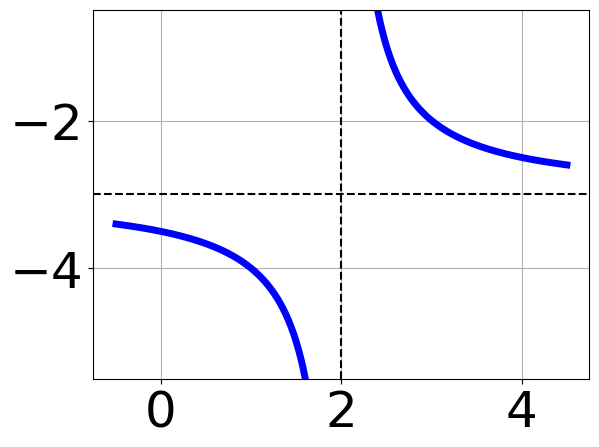
\includegraphics[width=0.5\textwidth]{../Figures/rationalGraphToEquationCopyB.png}
\end{center}



The solution is \( f(x) = \frac{-1}{(x + 3)^2} + 1 \), which is option D.\begin{enumerate}[label=\Alph*.]
\item \( f(x) = \frac{1}{(x - 3)^2} + 1 \)

Corresponds to using the general form $f(x) = \frac{a}{(x+h)^2}+k$ and the opposite leading coefficient.
\item \( f(x) = \frac{1}{x - 3} + 1 \)

Corresponds to thinking the graph was a shifted version of $\frac{1}{x}$, using the general form $f(x) = \frac{a}{(x+h)^2}+k$, and the opposite leading coefficient.
\item \( f(x) = \frac{-1}{x + 3} + 1 \)

Corresponds to thinking the graph was a shifted version of $\frac{1}{x}$.
\item \( f(x) = \frac{-1}{(x + 3)^2} + 1 \)

This is the correct option.
\item \( \text{None of the above} \)

This corresponds to believing the vertex of the graph was not correct.
\end{enumerate}

\textbf{General Comment:} Remember that the general form of a basic rational equation is $ f(x) = \frac{a}{(x-h)^n} + k$, where $a$ is the leading coefficient (and in this case, we assume is either $1$ or $-1$), $n$ is the degree (in this case, either $1$ or $2$), and $(h, k)$ is the intersection of the asymptotes.
}
\litem{
Solve the rational equation below. Then, choose the interval(s) that the solution(s) belongs to.
\[ \frac{-5x}{2x + 5} + \frac{-6x^{2}}{4x^{2} -4 x -35} = \frac{-3}{2x -7} \]
The solution is \( \text{There are two solutions: } x = -0.325 \text{ and } x = 2.887 \), which is option A.\begin{enumerate}[label=\Alph*.]
\item \( x_1 \in [-1.13, -0.11] \text{ and } x_2 \in [-2.11,3.89] \)

* $x = -0.325 \text{ and } x = 2.887$, which is the correct option.
\item \( x_1 \in [-1.13, -0.11] \text{ and } x_2 \in [-2.5,-1.5] \)


\item \( x \in [3.11,3.91] \)


\item \( \text{All solutions lead to invalid or complex values in the equation.} \)


\item \( x \in [2.58,3.27] \)


\end{enumerate}

\textbf{General Comment:} Distractors are different based on the number of solutions. Remember that after solving, we need to make sure our solution does not make the original equation divide by zero!
}
\litem{
Solve the rational equation below. Then, choose the interval(s) that the solution(s) belongs to.
\[ \frac{-48}{48x + 96} + 1 = \frac{-48}{48x + 96} \]
The solution is \( \text{all solutions are invalid or lead to complex values in the equation.} \), which is option E.\begin{enumerate}[label=\Alph*.]
\item \( x \in [-2.0,-1.0] \)

$x = -2.000$, which corresponds to not checking if this value leads to dividing by 0 in the original equation and thus is not a valid solution.
\item \( x_1 \in [-2, 0] \text{ and } x_2 \in [-3,0] \)

$x = -2.000 \text{ and } x = -2.000$, which corresponds to getting the correct solution and believing there should be a second solution to the equation.
\item \( x \in [2,5] \)

$x = 2.000$, which corresponds to not distributing the factor $48x + 96$ correctly when trying to eliminate the fraction.
\item \( x_1 \in [-2, 0] \text{ and } x_2 \in [1,3] \)

$x = -2.000 \text{ and } x = 2.000$, which corresponds to getting the correct solution and believing there should be a second solution to the equation.
\item \( \text{All solutions lead to invalid or complex values in the equation.} \)

*$x = -2.000$ leads to dividing by 0 in the original equation and thus is not a valid solution, which is the correct option.
\end{enumerate}

\textbf{General Comment:} Distractors are different based on the number of solutions. Remember that after solving, we need to make sure our solution does not make the original equation divide by zero!
}
\litem{
Choose the graph of the equation below.
\[ f(x) = \frac{-1}{(x - 2)^2} + 2 \]
The solution is the graph below, which is option E.
\begin{center}
    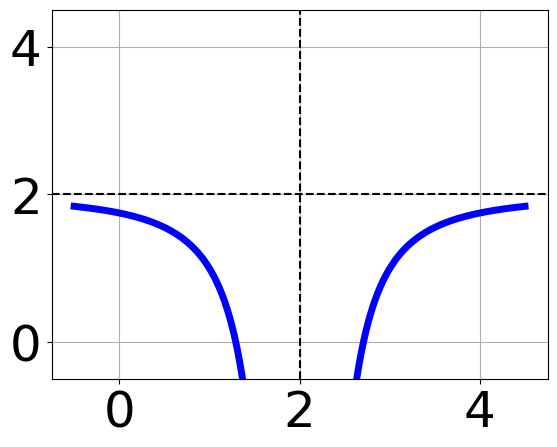
\includegraphics[width=0.3\textwidth]{../Figures/rationalEquationToGraphEB.png}
\end{center}\begin{enumerate}[label=\Alph*.]
\begin{multicols}{2}
\item 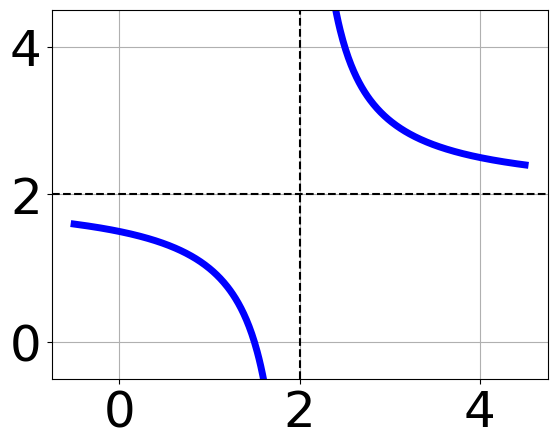
\includegraphics[width = 0.3\textwidth]{../Figures/rationalEquationToGraphAB.png}
\item 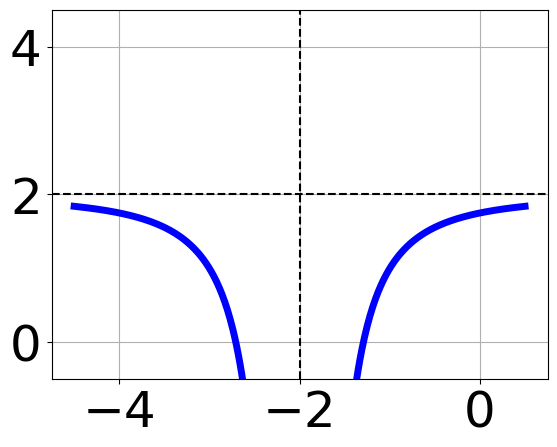
\includegraphics[width = 0.3\textwidth]{../Figures/rationalEquationToGraphBB.png}
\item 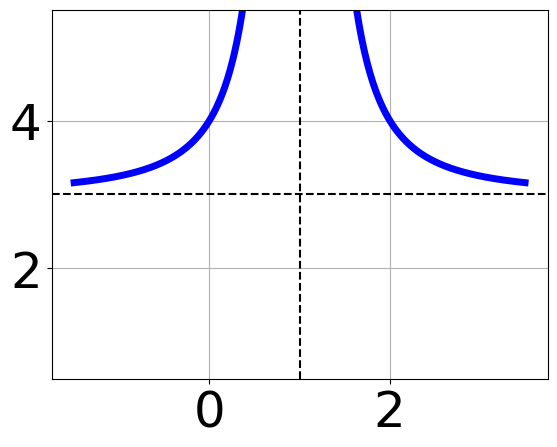
\includegraphics[width = 0.3\textwidth]{../Figures/rationalEquationToGraphCB.png}
\item 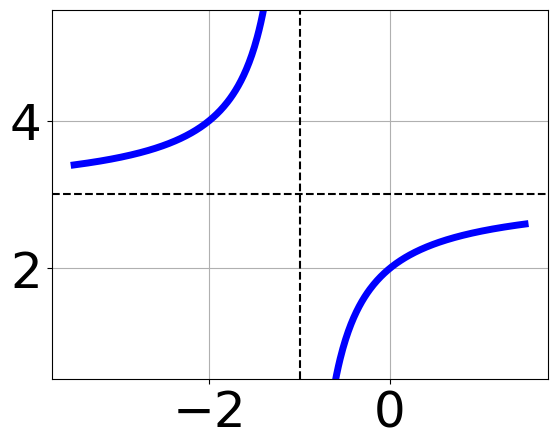
\includegraphics[width = 0.3\textwidth]{../Figures/rationalEquationToGraphDB.png}
\end{multicols}\item None of the above.\end{enumerate}
\textbf{General Comment:} Remember that the general form of a basic rational equation is $ f(x) = \frac{a}{(x-h)^n} + k$, where $a$ is the leading coefficient (and in this case, we assume is either $1$ or $-1$), $n$ is the degree (in this case, either $1$ or $2$), and $(h, k)$ is the intersection of the asymptotes.
}
\litem{
Choose the equation of the function graphed below.

\begin{center}
    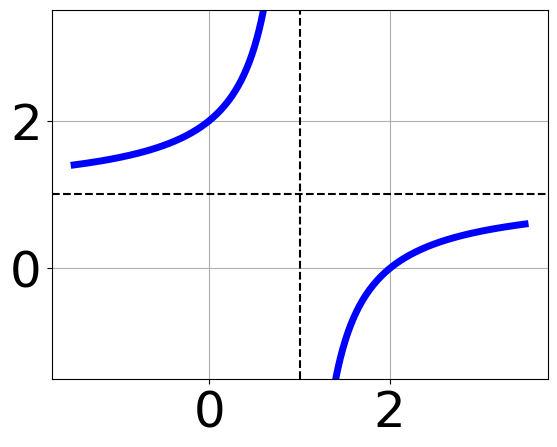
\includegraphics[width=0.5\textwidth]{../Figures/rationalGraphToEquationB.png}
\end{center}



The solution is \( f(x) = \frac{-1}{x - 1} + 1 \), which is option C.\begin{enumerate}[label=\Alph*.]
\item \( f(x) = \frac{-1}{(x - 1)^2} + 1 \)

Corresponds to thinking the graph was a shifted version of $\frac{1}{x^2}$.
\item \( f(x) = \frac{1}{(x + 1)^2} + 1 \)

Corresponds to thinking the graph was a shifted version of $\frac{1}{x^2}$, using the general form $f(x) = \frac{a}{x+h}+k$, and the opposite leading coefficient.
\item \( f(x) = \frac{-1}{x - 1} + 1 \)

This is the correct option.
\item \( f(x) = \frac{1}{x + 1} + 1 \)

Corresponds to using the general form $f(x) = \frac{a}{x+h}+k$ and the opposite leading coefficient.
\item \( \text{None of the above} \)

This corresponds to believing the vertex of the graph was not correct.
\end{enumerate}

\textbf{General Comment:} Remember that the general form of a basic rational equation is $ f(x) = \frac{a}{(x-h)^n} + k$, where $a$ is the leading coefficient (and in this case, we assume is either $1$ or $-1$), $n$ is the degree (in this case, either $1$ or $2$), and $(h, k)$ is the intersection of the asymptotes.
}
\litem{
Solve the rational equation below. Then, choose the interval(s) that the solution(s) belongs to.
\[ \frac{-3x}{-7x + 7} + \frac{-2x^{2}}{-42x^{2} +77 x -35} = \frac{7}{6x -5} \]
The solution is \( \text{There are two solutions: } x = 1.268 \text{ and } x = 1.932 \), which is option D.\begin{enumerate}[label=\Alph*.]
\item \( \text{All solutions lead to invalid or complex values in the equation.} \)


\item \( x \in [1.6,2.09] \)


\item \( x_1 \in [1.02, 1.36] \text{ and } x_2 \in [-0.7,1.8] \)


\item \( x_1 \in [1.02, 1.36] \text{ and } x_2 \in [1.6,2] \)

* $x = 1.268 \text{ and } x = 1.932$, which is the correct option.
\item \( x \in [0.72,0.94] \)


\end{enumerate}

\textbf{General Comment:} Distractors are different based on the number of solutions. Remember that after solving, we need to make sure our solution does not make the original equation divide by zero!
}
\litem{
Solve the rational equation below. Then, choose the interval(s) that the solution(s) belongs to.
\[ \frac{4}{-7x -9} + -7 = \frac{-5}{-63x -81} \]
The solution is \( x = -1.379 \), which is option A.\begin{enumerate}[label=\Alph*.]
\item \( x \in [-1.38,0.62] \)

* $x = -1.379$, which is the correct option.
\item \( x \in [1.13,1.22] \)

$x = 1.193$, which corresponds to not distributing the factor $-7x -9$ correctly when trying to eliminate the fraction.
\item \( x_1 \in [-1.49, -1.38] \text{ and } x_2 \in [-2.38,0.62] \)

$x = -1.469 \text{ and } x = -1.379$, which corresponds to getting the correct solution and believing there should be a second solution to the equation.
\item \( x_1 \in [-1.39, -1.28] \text{ and } x_2 \in [0.19,4.19] \)

$x = -1.379 \text{ and } x = 1.193$, which corresponds to getting the correct solution and believing there should be a second solution to the equation.
\item \( \text{All solutions lead to invalid or complex values in the equation.} \)

This corresponds to thinking $x = -1.379$ leads to dividing by zero in the original equation, which it does not.
\end{enumerate}

\textbf{General Comment:} Distractors are different based on the number of solutions. Remember that after solving, we need to make sure our solution does not make the original equation divide by zero!
}
\litem{
Choose the graph of the equation below.
\[ f(x) = \frac{1}{(x + 3)^2} + 3 \]
The solution is the graph below, which is option E.
\begin{center}
    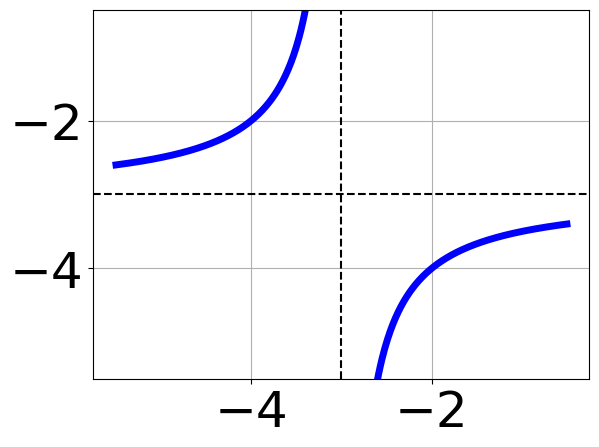
\includegraphics[width=0.3\textwidth]{../Figures/rationalEquationToGraphCopyEB.png}
\end{center}\begin{enumerate}[label=\Alph*.]
\begin{multicols}{2}
\item 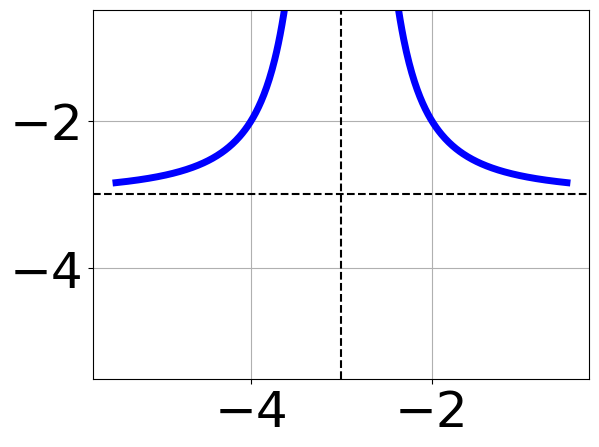
\includegraphics[width = 0.3\textwidth]{../Figures/rationalEquationToGraphCopyAB.png}
\item 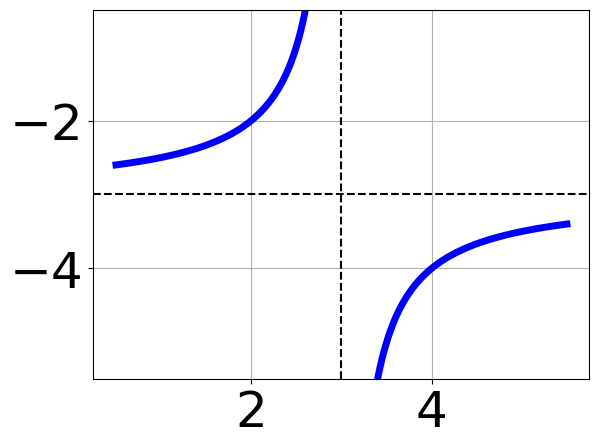
\includegraphics[width = 0.3\textwidth]{../Figures/rationalEquationToGraphCopyBB.png}
\item 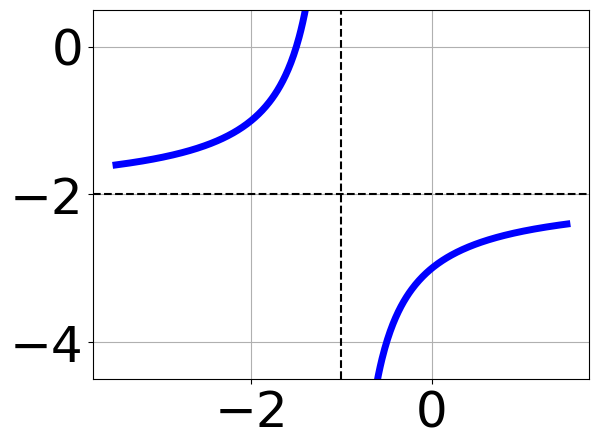
\includegraphics[width = 0.3\textwidth]{../Figures/rationalEquationToGraphCopyCB.png}
\item 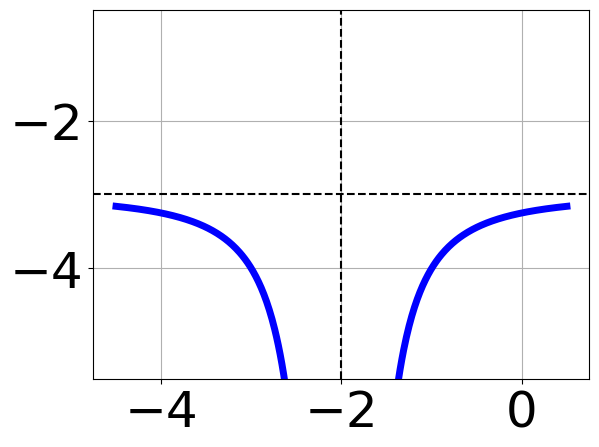
\includegraphics[width = 0.3\textwidth]{../Figures/rationalEquationToGraphCopyDB.png}
\end{multicols}\item None of the above.\end{enumerate}
\textbf{General Comment:} Remember that the general form of a basic rational equation is $ f(x) = \frac{a}{(x-h)^n} + k$, where $a$ is the leading coefficient (and in this case, we assume is either $1$ or $-1$), $n$ is the degree (in this case, either $1$ or $2$), and $(h, k)$ is the intersection of the asymptotes.
}
\end{enumerate}

\end{document}